\subsubsection{UC36 - Ricerca dizionari dati per nome}\label{UC36}

\begin{figure}[H]
  \centering
  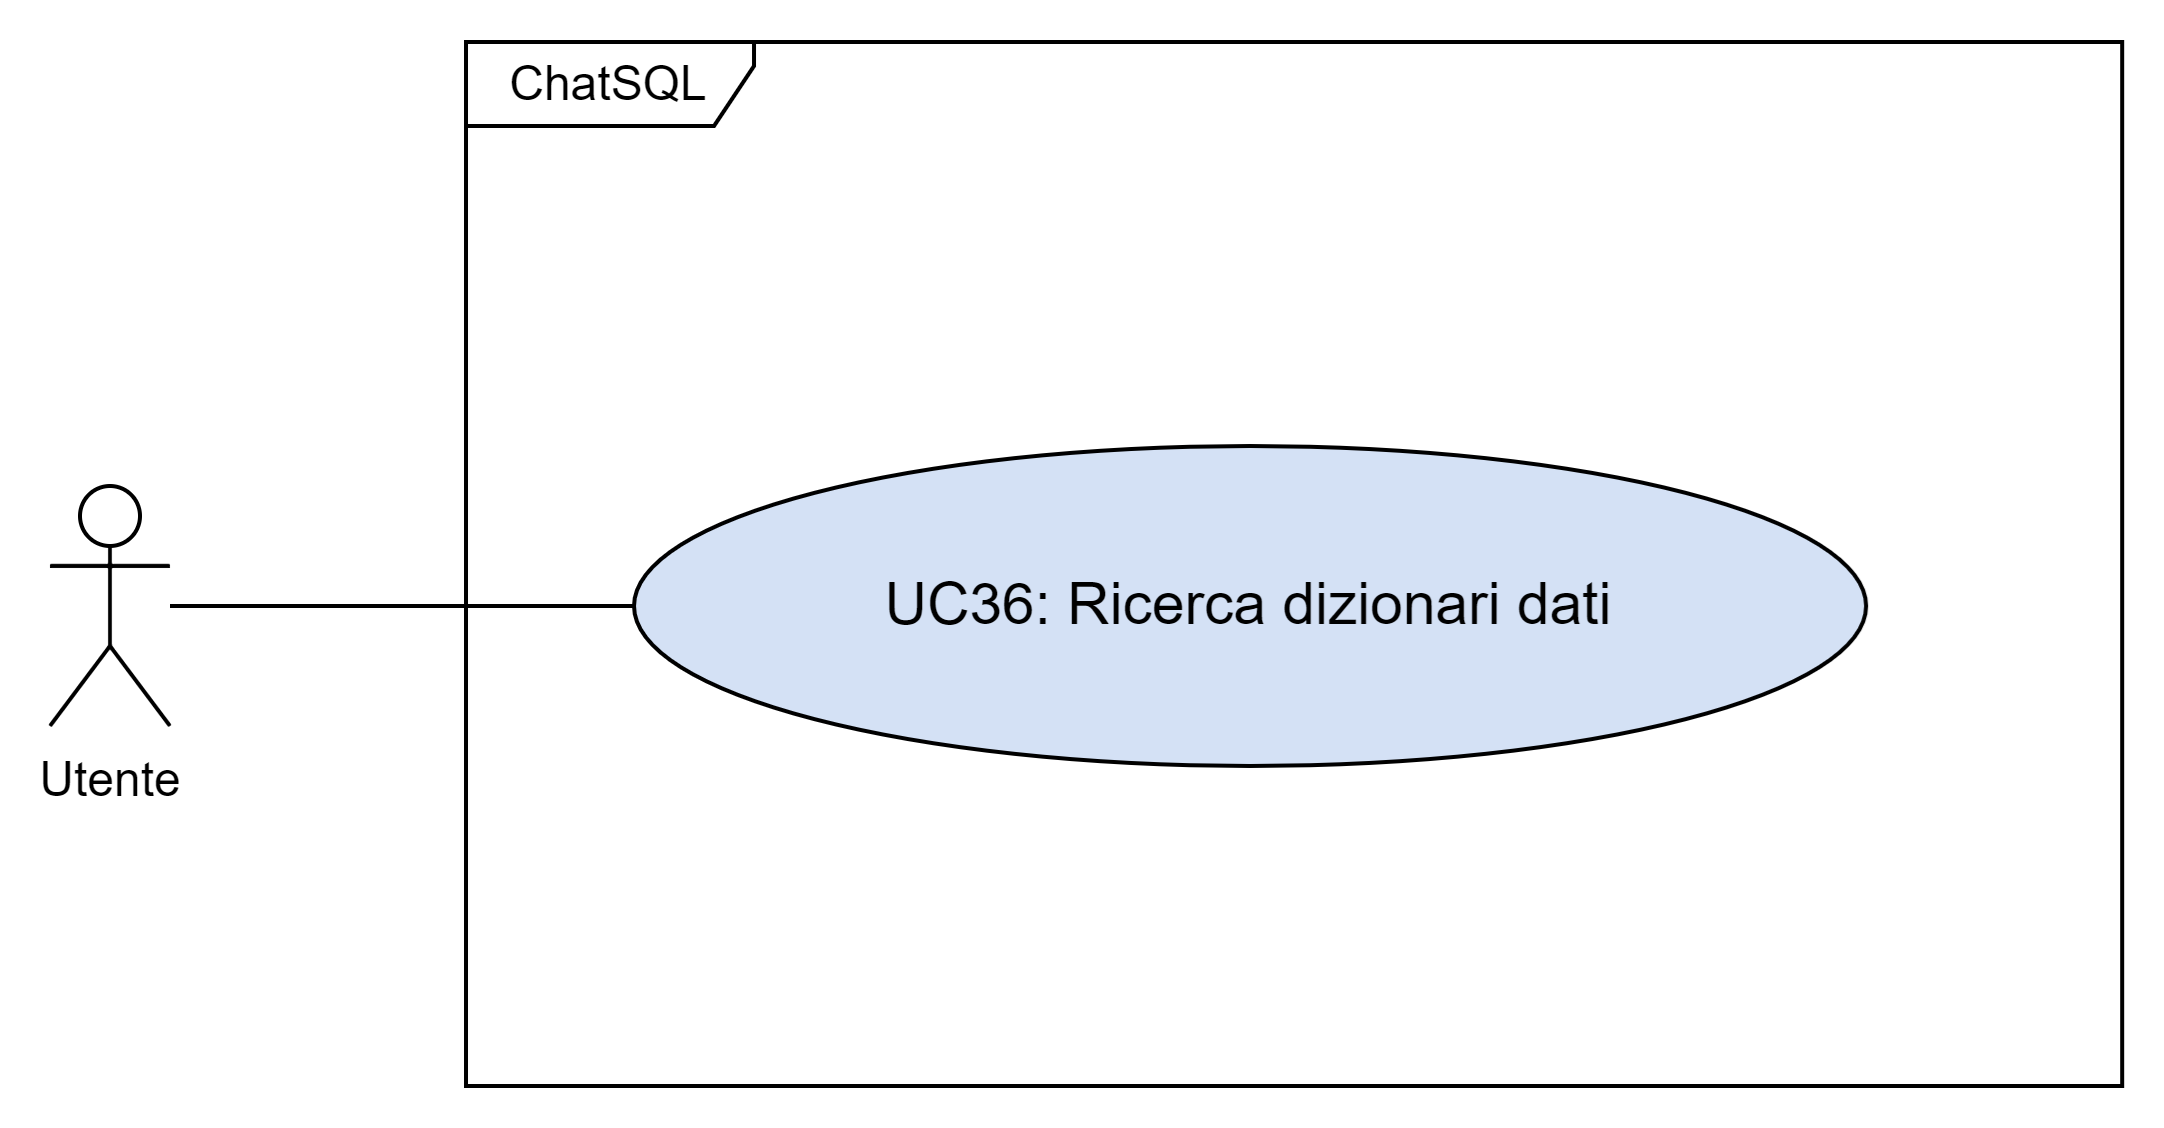
\includegraphics[width=0.90\textwidth]{assets/uc36.png}
  \caption{UC36}
\end{figure}

\paragraph*{Descrizione}
L'Utente effettua una ricerca per nome tra i \glossario{dizionari dati} presenti nel sistema.

\paragraph*{Attori principali}
Utente

\paragraph*{Precondizioni}
\begin{itemize}
  \item Il sistema è attivo e funzionante;
  \item L'Utente sta visualizzando la lista dei \glossario{dizionari dati} disponibili (\hyperref[UC9]{UC9}).
\end{itemize}

\paragraph*{Postcondizioni}
\begin{itemize}
  \item Vengono visualizzati i risultati della ricerca.
\end{itemize}

\paragraph*{Trigger}
L'Utente vuole filtrare i \glossario{dizionari dati} per nome.

\paragraph*{Scenario principale}
\begin{enumerate}
  \item L'Utente richiede al sistema di eseguire una ricerca per nome tra i \glossario{dizionari dati};
  \item Il sistema mostra i risultati della ricerca.
\end{enumerate}
